\documentclass[../../document.tex]{subfiles}
\begin{document}

\section*{Aufgabe 2}

\subsection*{a)}

\begin{equation*}
    \begin{split}
        \hat{u} &= \sqrt[]{2} * \SI{230}{\volt} = \SI{325}{\volt}\\
    \end{split}
\end{equation*}

\subsubsection*{I)}

\begin{equation*}
    \begin{split}
        \ubar{Z} &= R = \SI{200}{\ohm}\\
        U &= U\cind{R} = \SI{230}{\volt}\\
        I &= \frac{U}{R} = \frac{\SI{230}{\volt}}{\SI{200}{\ohm}} = \SI{1,15}{\ampere}\\
        \hat{i} &= \sqrt[]{2} *I = \SI{1,62}{\ampere}\\
    \end{split}
\end{equation*}

\begin{figure}[H]
    \begin{center}
        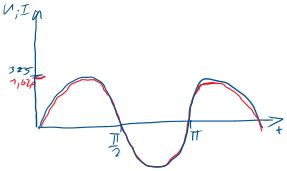
\includegraphics[width=.9\linewidth]{../../img/task1-a-i.jpeg}
    \end{center}
\end{figure}

\subsubsection*{II)}

\begin{equation*}
    \begin{split}
        \ubar{Z} &= X\cind{L} = j \omega * L = j \frac{U}{I} = j \frac{\SI{230}{\volt}}{\SI{2}{\ampere}} = j \SI{115}{\ohm}\\
        L &= \frac{X\cind{L}}{j\omega} = \frac{j \SI{115}{\ohm}}{j \SI{50}{\hertz}} = \SI{0,366}{\henry}\\
        U &= U\cind{P} = \SI{230}{\volt}\\
        \hat{i} &= \sqrt[]{2} * I = \SI{2,84}{\ampere}\\
        \hat{u} &= \sqrt[]{2} * U = \SI{325}{\volt}\\
    \end{split}
\end{equation*}

\begin{figure}[H]
    \begin{center}
        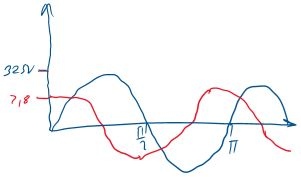
\includegraphics[width=.9\linewidth]{../../img/task1-a-ii.jpeg}
    \end{center}
\end{figure}

\subsubsection*{III)}

\begin{equation*}
    \begin{split}
        \ubar{Z} &= X\cind{C} = \frac{1}{j \omega * L} = j \frac{U}{I} = j \frac{\SI{230}{\volt}}{\SI{0,5}{\ampere}} = j \SI{460}{\ohm}\\
        C &= \frac{X\cind{C}}{j\omega} = \frac{j \SI{460}{\ohm}}{j \SI{50}{\hertz}} = \SI{9,2}{\farad}\\
        U &= U\cind{P} = \SI{230}{\volt}\\
        \hat{i} &= \sqrt[]{2} * I = \SI{0,707}{\ampere}\\
        \hat{u} &= \sqrt[]{2} * U = \SI{325}{\volt}\\
    \end{split}
\end{equation*}

\begin{figure}[H]
    \begin{center}
        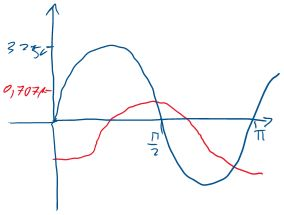
\includegraphics[width=.9\linewidth]{../../img/task1-a-iii.jpeg}
    \end{center}
\end{figure}

\subsection*{b)}

\begin{equation*}
    \begin{split}
        P &= Re\left[\ubar{S}\right] = Re\left[U * I * e^{j * (\varphi\cind{u} - \varphi\cind{i})}\right] = U * I * cos(\varphi\cind{u} - \varphi\cind{i})\\
        Q &= Im\left[\ubar{S}\right] = Im\left[U * I * e^{j * (\varphi\cind{u} - \varphi\cind{i})}\right] = U * I * sin(\varphi\cind{u} - \varphi\cind{i})\\
        S &= \frac{1}{2} * \ubar{\hat{u}} * \ubar{\hat{i}}^* = \ubar{U} * \ubar{I}^*
    \end{split}
\end{equation*}

\subsubsection*{I)}

\begin{equation*}
    \begin{split}
        P &= U * I * cos(\varphi) \textrm{ mit } \varphi = 0\textrm{ da realer Widerstand}\\
        &= \SI{230}{\volt} * \SI{1,15}{\ampere} * cos(0) = \SI{264,5}{\watt}\\\\
        S &= P\\
    \end{split}
\end{equation*}

\subsubsection*{II)}

\begin{equation*}
    \begin{split}
        P &= 0\textrm{ da ideal}\\
        Q &= U * I * sin(\varphi) \textrm{ mit } \varphi = \SI{90}{\degree}\textrm{ da Induktivität}\\
        &= \SI{230}{\volt} * \SI{2}{\ampere} * sin(\SI{90}{\degree}) = \SI{480}{var}\\
        S &= Q\\
    \end{split}
\end{equation*}

\subsubsection*{III)}

\begin{equation*}
    \begin{split}
        P &= 0\textrm{ da ideal}\\
        Q &= U * I * sin(\varphi) \textrm{ mit } \varphi = \SI{-90}{\degree}\textrm{ da Kondensator}\\
        &= \SI{230}{\volt} * \SI{0,5}{\ampere} * sin(\SI{-90}{\degree}) = \SI{-150}{var}\\
        S &= Q\\
    \end{split}
\end{equation*}

\subsection*{c)}

\subsubsection*{I)}

\begin{equation*}
    \begin{split}
        W\cind{Q} &= 0\\
        W\cind{P} &= P * h = \SI{264,5}{\watt} * \SI{4}{\hour} = \SI{1058}{\frac{\watt}{\hour}}\\
    \end{split}
\end{equation*}

\subsubsection*{II)}

\begin{equation*}
    \begin{split}
        W\cind{Q} &= Q * h = \SI{480}{var} * \SI{4}{\hour} = \SI{1920}{\frac{var}{\hour}}\\
        W\cind{P} &= 0\\
    \end{split}
\end{equation*}

\subsubsection*{III)}

\begin{equation*}
    \begin{split}
        W\cind{Q} &= Q * h = \SI{-115}{var} * \SI{4}{\hour} = \SI{-460}{\frac{var}{\hour}}\\
        W\cind{P} &= 0\\
    \end{split}
\end{equation*}

\subsection*{d)}

\begin{equation*}
    \begin{split}
        W\cind{P} &= W\cind{P,I} = \SI{1058}{\frac{\watt}{\hour}} \\
        W\cind{Q} &= W\cind{Q,II} + W\cind{Q,II} = \SI{1920}{\frac{var}{\hour}} - \SI{460}{\frac{var}{\hour}} = \SI{1460}{\frac{var}{\hour}}
    \end{split}
\end{equation*}

\subsection*{e)}

\begin{equation*}
    \begin{split}
        \ubar{S} &= \sqrt[]{1058^2 + (1920 - 460)^2} = \SI{1803,04}{\volt\ampere}\\
        \ubar{I} &= \frac{\ubar{S}}{\ubar{U}} = \frac{\SI{1803,04}{\volt\ampere}}{\SI{230}{\volt}} = \SI{7,84}{\ampere}\\
        \varphi &= arccos\left(\frac{P}{S}\right) = arccos\left(\frac{\SI{1058}{\watt}}{\SI{1803,04}{\volt\ampere}}\right) = \SI{54,07}{\degree}\\
    \end{split}
\end{equation*}

\subsection*{f)}

\begin{figure}[H]
    \begin{center}
        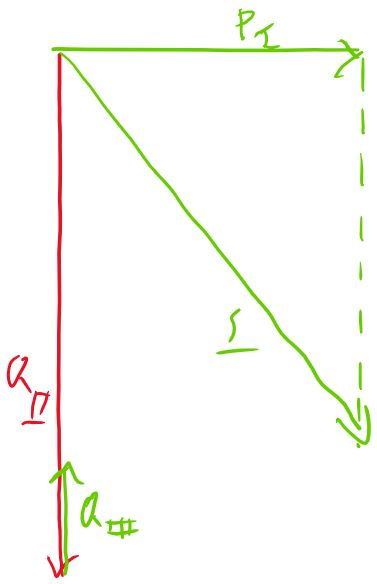
\includegraphics[width=.9\linewidth]{../../img/task1-f.jpeg}
    \end{center}
\end{figure}

\end{document}